\documentclass{article}

\usepackage{ulem}
\usepackage{amsmath}
\usepackage{graphicx}
\usepackage{geometry}
\usepackage{hyperref}
\usepackage{color}
\usepackage{listings}
\lstset{ % General setup for the package
    language=Python,
    basicstyle=\small\ttfamily,
    numbers=left,
     numberstyle=\tiny,
    frame=tb,
    tabsize=4,
    columns=fullflexible,
    breaklines=true,
    postbreak=\mbox{\textcolor{red}{$\hookrightarrow$}\space},
    showstringspaces=false,
    showtabs=false,
    keepspaces,
    commentstyle=\color{red},
    keywordstyle=\color{blue}
}

\title{Lecture 2 Project: Document Distance}
\author{Yanuar Heru Prakosa}
\date{31-05-2021}

\begin{document}
    \maketitle

    \section*{The Document Distance}
    The assignment from the Lecture 2 in 6-006 is related to one called document distance. 
    Thus I need to find out first what is exactly document distance is.  
    \href{http://6.006.scripts.mit.edu/~6.006/spring08/wiki/index.php?title=Document_Distance_Problem_Definition}{Form this MIT discussion webpage}, I learn that document distance will be measured using vector equations.
    Let D be a text, then a word is a consecutive of alphanumeric characters. 
    We will not distinguish upper case and lower case letters, but we use non alphanumeric characters as delimiter between words.
    For example the word "can't" consist of 2 words: can and t.
    
    Okay now we go to the formulation:
    The word \emph{word frequency distribution} of a document D ia a mapping from words \emph{w} to their frequency count, denoted as $D(w)$.
    We can view the frequency distribution D as vector, with one component per possible word. Each component will be a non-negative integer $\geq 0$.

    The norm of this vector is defined by:
    \begin{equation*}
        N(D) = \sqrt{D \cdot D} = \sqrt{\sum_{w}{D(w)^{2}}}
    \end{equation*}
    Alright this calculation still does not make any sense right now.
    But let's move on, I need to get to how to calculate document distance first.
    Now when we have two documents to be compared to each other, let's name them $D$ and $D'$. 
    The inner product between $D$ and $D'$ is defined as:
    \begin{equation*}
        D \cdot D' = \sum_{w}{D(w)D'(w)}
    \end{equation*}
    So basically this is the sum of products on all word frequencies in two documents.
    Thus, if a word exist 1000 times in one document but never existed in other document the inner product of that part is 0!

    Okay, since our objective is to define distance which is defined here as angle between two documents we need to go back to definition of vector dot products:
    \begin{equation*}
        D \cdot D' = N(D) N(D') cos \theta
    \end{equation*}
    As we looking for an angle we are focusing on $\theta$ right?
    Therefore:
    \begin{equation*}
        cos \theta = \frac{D \cdot D'}{N(D)N(D')}
    \end{equation*}
    \begin{equation*}
        \theta = arccos \left( \frac{D \cdot D'}{N(D)N(D')} \right)
    \end{equation*}
    Deriving from other equations above we will get:
    \[
      \theta = arccos \left( \frac{\sum_{w}{D(w)D'(w)}}{\sqrt{\sum_{w}{D(w)^{2}}} \sqrt{\sum_{w}{D'(w)^{2}}}}\right)  
    \]
    From those formula we can infer that if both Documents are the same then the $angle(D,D') = \theta = 0$.
    On the other hand if both documents are completely different in the sense there are no similarity in terms of word used in it then the $angle(D,D') = \theta = \frac{\pi}{2}$. Please note we are using \emph{radians} in this matter.

    \section*{Pre Example}
    To make it clearer I think a simple practical example is mandatory. 
    Let us have two sentences that we will use as documents. 
    One is "To be or not to be" and the other is "Doubt truth to be a liar". 
    We will calculate the distance between these two documents.

    Now we already list all unique set of words and it can be seen in this table plus its frequencies:
    \begin{center}
        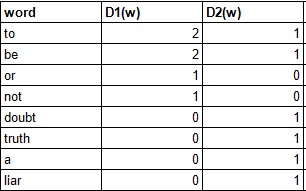
\includegraphics{table word frequencies}    
    \end{center}
        
    Now let's get back to the formula: 
    \[
      \theta = arccos \left( \frac{\sum_{w}{D(w)D'(w)}}{\sqrt{\sum_{w}{D(w)^{2}}} \sqrt{\sum_{w}{D'(w)^{2}}}}\right)  
    \]
    we begin with the denominator part first.

    \newpage
    To calculate the denominator we need to find $\sum_{w}{D(w)^{2}}$ and $\sum_{w}{D'(w)^{2}}$ first. Here is the results of the calculation:
    \begin{center}
        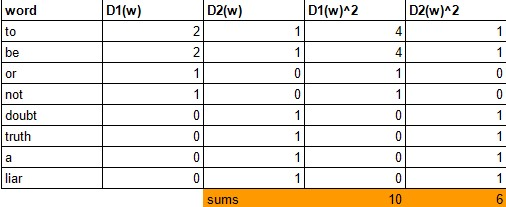
\includegraphics{square frequencies table.jpg}
    \end{center}

    As you can see the sums already being included in the table above.
    We can use it as our denominators, but remember those sum products must be subject to a square root operations.
    Now we need to calculate the nominator side: $sum{D(w)D'(W)}$, which we have already calculated also using spreadsheet:
    \begin{center}
        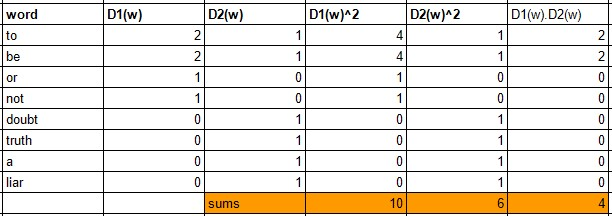
\includegraphics[scale=0.8]{inner product sum table.jpg}
    \end{center}

    As you can see on the table above the $sum{D(w)D'(W)} = 4$, now we can put all of them in the formula:
    \[\theta = arccos \left( \frac{4}{\sqrt{10} \sqrt{6}}\right)\]
    \[\theta = arccos \left( \frac{4}{\sqrt{10.6}}\right)\]
    \[\theta = arccos\left( 0.52\right)\]
    \[\theta = 1.028157225\]

    There you are, that is in summary how we will measure the distance between to documents. 

    \section*{Summary}
    Here is what you should do when measuring the distance between two documents:
    \begin{enumerate}
        \item list all words in a set, meaning there are no double words in a set all words are unique
        \item count the frequency of occurance for each word in each document (WARNING: EACH NOT TOTAL)
        \item use vector inner product and normalization also dot products to calculate the angle (SEE THE FORMULAS AND EXAMPLE ABOVE)
        \item that angle when is closer to 0 (the minimum angle is 0) then the chance both documents are the same is higher (some use this as an indication of plagiarism)
        \item Vice versa when the angle is closer towards $\frac{\pi}{2}$ then the documents are less similar.
        \item Just remember this is only a basic algorithm on how to measure document distance, many ways can be used to cheat this algorithm thus this kind of measurements always evolving in terms of algorithms. 
        \item Stay tune and keep learning!
    \end{enumerate}
    \newpage
    \section{Coding in Python}
    Now after we know how to formulate the document distance, we can start use it to formulate pseudocode. 
    The algorithm will be mesured after the pseudocode is implemented into code in python.
    Each python file here uses different algorithm or should I say method on how to handle the words inside the documents.
    These words are what used to measure the document distance later on using vector normalized multiplication.

    Well it is better if we research each python file to understand the way they were calculated. 
    I need to have method in order to debug the code later on to make sense of the algorithms they use.
    However, preparing method to debug the code is not as simple as it might sounds.
    For once the built in VSCode debugger does not allow the *args input from the user. 
    Meanwhile the Python own debug library is lacking in the user interface features.

    If I need to choose between the two, right now I more lean towards the VSCode internal debugger. 
    I must make some adjustment in the main function in order to put the *args into the system. 
    I need to make the test document (t1 and t2) still passed into the argument after the main function is called.
    \begin{lstlisting}
        def main():
            if len(sys.argv) != 3:
                print ("Usage: docdist1.py filename_1 filename_2")
            else:
                filename_1 = sys.argv[1]
                filename_2 = sys.argv[2]
                sorted_word_list_1 = word_frequencies_for_file(filename_1)
                sorted_word_list_2 = word_frequencies_for_file(filename_2)
                distance = vector_angle(sorted_word_list_1,sorted_word_list_2)
                print ("The distance between the documents is: %0.6f (radians)"%distance)
    \end{lstlisting}
    As you can see in the main function if the user does not include additional arguments in the CLI when invoking the docdist program it will invoke warning and stop the program altogether.
    In order to solve this problem I need to make the run will include the t1.verne.txt and t2.bobsey.txt in the initial parameters.
    Why we use t1.verne.txt and t2.bobsey.txt? Well because both files are the smallest of all documents in the project.
    This is merely a test run and debug run to see how the code works.
    Thus, choosing the smallest file as example for all docdist program (docdist1 to docdist6) will result comparable and comprehensive results.

    In order to make the VSCode built in debugger works I need to modify the main function a bit. 
    The main idea here is to make the test documents files part of the arguments from the first time debug run is initiated.
    As we cannot use CLI to run the debug state of the program then I need to modify the main function as this is the function called first on run.
    Here is the modification of the code:
    \begin{lstlisting}
        def main():
    # import pdb; pdb.set_trace() # <--- this is for debug purpose only
    if len(sys.argv) != 3:
        print ("Usage: docdist4.py filename_1 filename_2")
        #-- FOR DEBUG PURPOSES ONLY
        filename_1 = 'E:\\python_me\\6-006_python\\lec02_code\\t1.verne.txt'
        filename_2 = 'E:\\python_me\\6-006_python\\lec02_code\\t2.bobsey.txt'
        sorted_word_list_1 = word_frequencies_for_file(filename_1)
        sorted_word_list_2 = word_frequencies_for_file(filename_2)
        distance = vector_angle(sorted_word_list_1,sorted_word_list_2)
        print ("The distance between the documents is: %0.6f (radians)"%distance)
        # --- comment out this after finish debugging!
    else:
        filename_1 = sys.argv[1]
        filename_2 = sys.argv[2]
        sorted_word_list_1 = word_frequencies_for_file(filename_1)
        sorted_word_list_2 = word_frequencies_for_file(filename_2)
        distance = vector_angle(sorted_word_list_1,sorted_word_list_2)
        print ("The distance between the documents is: %0.6f (radians)"%distance)
    \end{lstlisting}
    NOTE: the file paths are in Windows format since the files are stored in the local Windows storage. 
    I think it will be safer to use Windows path format.

    \subsection{UML Sequence Diagram}
    I need tool to help me understand how the program works. 
    As takin notes are too random and the contents are easier to forget, I think I need better methods to make sense how the program works.
    The Sequence Diagram from UML sounds like a good tool for this job. 
    Unlike static Class Diagram the Sequence Diagram will record the interaction between function(?) in the program.

    \subsection{Docdist1}
    In the docdist 1 there is a specification at this:
    \begin{lstlisting}
        #!/usr/bin/python
        # docdist1.py - initial version of document distance
        #
        # Original version by Ronald L. Rivest on February 14, 2007
        # Revision by Erik D. Demaine on September 12, 2011
        #
        # Usage:
        #    docdist1.py filename1 filename2
        #     
        # This program computes the "distance" between two text files
        # as the angle between their word frequency vectors (in radians).
        #
        # For each input file, a word-frequency vector is computed as follows:
        #    (1) the specified file is read in
        #    (2) it is converted into a list of alphanumeric "words"
        #        Here a "word" is a sequence of consecutive alphanumeric
        #        characters.  Non-alphanumeric characters are treated as blanks.
        #        Case is not significant.
        #    (3) for each word, its frequency of occurrence is determined
        #    (4) the word/frequency lists are sorted into order alphabetically
        #
        # The "distance" between two vectors is the angle between them.
        # If x = (x1, x2, ..., xn) is the first vector (xi = freq of word i)
        # and y = (y1, y2, ..., yn) is the second vector,
        # then the angle between them is defined as:
        #    d(x,y) = arccos(inner_product(x,y) / (norm(x)*norm(y)))
        # where:
        #    inner_product(x,y) = x1*y1 + x2*y2 + ... xn*yn
        #    norm(x) = sqrt(inner_product(x,x))

    \end{lstlisting}
    I must admit the specification is a bit long, but this is important since these specifications will be the basis to compare to other algorithms.
    The basic principle here is:
    \begin{enumerate}
        \item read all the lines in both documents that will return list of strings per line in document
        \item from all of those list of strings they were split into words, hence return list of words.
        \item then calculate the frequency of each word and put it into list in a list ie: [['0', 3],['an', 42]], means the string zero has 3 times occurance while string word an has 42 occurrance in one document.
        \item then sort them alphabetically, NOT based on frequency value.
        \item then begin finding vector distance using dot based inner products.
    \end{enumerate}
    Basically, the final steps will be similar across the Docdist algorithms. 
    However, minor changes might prove useful to increase the processing speed. 
    For the docdist1.py the processing time is 3.625 with document distance = 0.582 radians.

    \subsection{Docdist2}
    Now in the Docdist2 there is only one small modification as stated in the top part of its specification:
    \begin{lstlisting}
        #!/usr/bin/python
        # docdist2.py - changed concatenate to extend in get_words_from_line_list
    \end{lstlisting}
    In the code at the \textbf{get\_words\_from\_line\_list} it is stated that using the List module extend function will make the process more efficient. 
    The List.extend(List:seq) is a fucntion that will add element of another list into the List that call it. 
    Other steps are basically the same as the Docdist1.py.
    However, just by modifying one line it has increase the computation speed.
    For docdist2.py the processing time is 3.188 seconds with document distance = 0.582 radians.
    
\end{document}